% ======================================================================================
% Nom     : reports/latex/main.tex
% Rôle    : Fichier principal du rapport LaTeX, assemble la page de garde, les sections et la bibliographie.
% Auteur  : Maxime BRONNY
% Version : V1
% Cadre   : Réalisé dans le cadre du cours Techniques d'apprentissage artificiel
%           Master 1 Informatique Big Data
% Usage   : Compiler avec latexmk -pdf main.tex depuis le dossier reports/latex.
% ======================================================================================

% ============================================================================
% Rapport de projet - Techniques d'Apprentissage Artificiel (M1)
% Prédiction du Risque de Crédit Bancaire (pipeline Python from scratch)
%
% Compilation (bibliographie intégrée, bibtex non requis) :
%   pdflatex main.tex && pdflatex main.tex
% ou, si latexmk est installé :
%   latexmk -pdf main.tex
% ============================================================================

\documentclass[11pt,a4paper]{article}

% ===== Encodage, langue et police (Latin Modern, rendu LaTeX classique) =====
\usepackage[utf8]{inputenc}
\usepackage[T1]{fontenc}
\usepackage[french]{babel}
\usepackage{lmodern}
\usepackage{microtype}            % micro-ajustements typographiques (gris plus régulier)

% Titres en français : « Sommaire » et « Bibliographie »
\addto\captionsfrench{\renewcommand{\contentsname}{Sommaire}}
\addto\captionsfrench{\renewcommand{\refname}{Bibliographie}}

% ===== Mise en page =====
\usepackage[margin=2.5cm,headheight=14pt]{geometry}
\usepackage{setspace}
\onehalfspacing
% Paragraphes en bloc (sans alinéa, séparés par un peu d'espace), pour un rendu
% plus aéré et plus homogène, conforme au style du rapport de référence.
\setlength{\parindent}{0pt}
\setlength{\parskip}{0.45em}
\usepackage{array}                % modificateurs de colonnes >{...} et \extrarowheight
\usepackage{longtable}            % glossaire aligné sur deux colonnes, multi-pages
\usepackage{enumitem}             % espacement homogène et sobre des listes
\setlist[itemize]{label=-, topsep=0.35em, itemsep=0.25em, parsep=0pt, leftmargin=1.6em}
\setlist[enumerate]{topsep=0.35em, itemsep=0.25em, parsep=0pt, leftmargin=1.8em}

% ===== Figures et tableaux =====
\usepackage{graphicx}
\usepackage{eso-pic}              % image de couverture en pleine page (A4)
% Les figures sont lues directement depuis les sorties du programme :
%   reports/figures/        : figures générées par python3 main.py
%   data/stats/             : figures d'exploration des données (EDA)
%   reports/latex/figures/  : figures propres au rapport (schémas, etc.)
\graphicspath{{../figures/}{figures/}{../../data/stats/}}
\usepackage{booktabs}
\usepackage{multirow}
\usepackage{float}
\usepackage{caption}
% Séparateur de légende en tiret simple : « Table 1 - ... » (et non « Table 1 – ... »)
\DeclareCaptionLabelSeparator{tiret}{ - }
\captionsetup{font=small,labelfont=bf,margin=0.8cm,labelsep=tiret}
% Espacement sobre et homogène autour des figures et tableaux.
\setlength{\textfloatsep}{1.2em}
\setlength{\floatsep}{1em}
\setlength{\intextsep}{1em}

% ===== Maths =====
\usepackage{amsmath,amssymb}

% ===== Titres de sections : centrés, avec une ligne pleine largeur dessous =====
\usepackage{titlesec}
% Chaque grande partie commence sur une nouvelle page. On n'ajoute PAS de
% \vspace* au-dessus du titre : en haut de page, un \vspace* fait basculer le
% titre sur une « deuxième ligne » et lui ajoute \topskip + une interligne
% complète (~1 cm de blanc en trop). Sans lui, le titre est la première ligne
% et reste haut, à une distance équilibrée de l'en-tête (~1,2 cm), proche du
% modèle visuel souhaité.
\newcommand{\sectionbreak}{\clearpage}
% Titre principal centré, suivi d'un filet fin sur toute la largeur du texte.
% Espaces équilibrés : titre -> filet (0.6em), puis filet -> texte (1.7em).
\titleformat{\section}[block]
  {\LARGE\bfseries\filcenter}     % grand, gras, centré
  {\thesection.}{0.6em}{}         % numéro . puis titre
  [{\vspace{0.6em}\titlerule[0.6pt]}]   % ligne horizontale pleine largeur
\titlespacing*{\section}{0pt}{0pt}{1.7em}
% Sous-sections et sous-sous-sections : sobres, alignées à gauche, numéro suivi
% d'un point (homogène avec les sections), bien détachées du paragraphe précédent.
\titleformat{\subsection}{\large\bfseries}{\thesubsection.}{0.6em}{}
\titlespacing*{\subsection}{0pt}{1.7em}{0.7em}
\titleformat{\subsubsection}{\normalsize\bfseries}{\thesubsubsection.}{0.6em}{}
\titlespacing*{\subsubsection}{0pt}{1.3em}{0.5em}

% ===== En-têtes et pieds de page =====
\usepackage{fancyhdr}
\pagestyle{fancy}
\fancyhf{}
\fancyhead[L]{\small UE - Techniques d'apprentissage artificiel}
\fancyhead[R]{\small Master 1 Big Data - Université Paris 8}
\fancyfoot[C]{\thepage}
\renewcommand{\headrulewidth}{0.4pt}
\renewcommand{\footrulewidth}{0pt}

% ===== Liens et code =====
\usepackage[hidelinks]{hyperref}
\usepackage{xurl}                 % coupe proprement les URL longues de la bibliographie
\usepackage{listings}
\lstset{
  language=Python,
  basicstyle=\ttfamily\small,
  keywordstyle=\bfseries,
  showstringspaces=false,
  frame=single,
  breaklines=true,
  literate={é}{{\'e}}1 {è}{{\`e}}1 {à}{{\`a}}1 {ç}{{\c{c}}}1 {ê}{{\^e}}1
           {î}{{\^\i}}1 {ô}{{\^o}}1 {û}{{\^u}}1 {É}{{\'E}}1 {È}{{\`E}}1
}

\begin{document}

% Puces de liste en tiret simple (le français babel utilise sinon un tiret long).
\renewcommand{\labelitemi}{-}
\renewcommand{\labelitemii}{-}
\renewcommand{\labelitemiii}{-}

% ============================================================================
% Page de garde
% ============================================================================
\begin{titlepage}
  % Couverture : page de présentation graphique (image A4 pleine page).
  % L'ancienne page de garde LaTeX est conservée dans l'historique git.
  \AddToShipoutPictureBG*{\AtPageLowerLeft{%
    
\includegraphics[width=\paperwidth,height=\paperheight]{page_de_presentation.png}}}
  \null
\end{titlepage}

% ============================================================================
% Pages liminaires : sommaire puis glossaire (numérotation romaine)
% ============================================================================
\pagenumbering{roman}
\tableofcontents

% ======================================================================================
% Nom     : reports/latex/sections/00_glossaire.tex
% Rôle    : Liste des sigles et glossaire des termes employés dans le rapport.
% Auteur  : Maxime BRONNY
% Version : V1
% Cadre   : Réalisé dans le cadre du cours Techniques d'apprentissage artificiel
%           Master 1 Informatique Big Data
% Usage   : Fichier inclus dans main.tex lors de la compilation du rapport.
% ======================================================================================

% ============================================================================
% Liste des sigles et glossaire - termes et acronymes réellement employés dans
% le rapport, classés par ordre alphabétique (terme à gauche, définition à
% droite). Page liminaire référencée dans le sommaire.
%
% Mise en page : longtable à deux colonnes sans filets (terme en gras à gauche,
% définition alignée à droite), qui se répartit proprement sur plusieurs pages
% et réserve toujours la hauteur de la ligne (pas de chevauchement).
% ============================================================================
\clearpage
\section*{Liste des sigles et glossaire}
\addcontentsline{toc}{section}{Liste des sigles et glossaire}

\begingroup
\setlength{\extrarowheight}{0.35em}   % respiration verticale entre les entrées
\begin{longtable}{@{}>{\raggedright\bfseries}p{3.2cm}@{\hspace{0.4cm}}>{\raggedright\arraybackslash}p{\dimexpr\textwidth-3.7cm\relax}@{}}

Accuracy & Exactitude : proportion de prédictions correctes, toutes classes
  confondues, $(TP+TN)/N$. Peu informative seule sur des données déséquilibrées. \\

Apprentissage supervisé & Famille de méthodes qui apprennent à prédire une
  variable cible à partir d'exemples étiquetés. \\

Arbre de décision & Modèle qui partitionne récursivement les données par des
  tests binaires « variable $\leq$ seuil » et prédit, dans chaque feuille, la
  proportion de défauts observée (voir CART). \\

AUC & \emph{Area Under the Curve} : aire sous la courbe ROC ; probabilité qu'un
  défaut tiré au hasard reçoive un score plus élevé qu'un non-défaut
  ($0{,}5$~=~hasard, $1$~=~classement parfait). \\

CART & \emph{Classification And Regression Tree} : algorithme d'arbre de décision
  fondé sur des séparations binaires successives des données. \\

Classification binaire & Tâche supervisée où la cible ne prend que deux
  valeurs ; ici, $0$~=~remboursement, $1$~=~défaut de paiement. \\

Courbe ROC & Courbe du taux de vrais positifs en fonction du taux de faux
  positifs lorsque le seuil de décision varie (voir ROC, AUC). \\

Dataset & Jeu de données : ensemble des observations disponibles ; ici,
  32\,581 dossiers de crédit décrits par 11 variables et une cible. \\

Descente de gradient & Algorithme d'optimisation itératif qui ajuste les
  paramètres dans la direction qui fait le plus baisser la fonction de coût. \\

Encodage & Conversion des variables catégorielles en nombres ; nous utilisons un
  \emph{label encoding} à correspondance fixe. \\

F1-score & Moyenne harmonique de la précision et du rappel ; critère de
  sélection des hyperparamètres dans ce projet. \\

Faux négatif (FN) & Défaut réel non détecté (crédit accordé à un client qui ne
  remboursera pas) : l'erreur la plus coûteuse pour la banque. \\

Faux positif (FP) & Bon client classé à tort comme défaut (crédit refusé sans
  raison réelle). \\

FN & \emph{Faux négatif} : voir Faux négatif. \\

FP & \emph{Faux positif} : voir Faux positif. \\

From scratch & Implémenté à partir des opérations de base (NumPy), sans
  bibliothèque d'apprentissage automatique. \\

Fuite de données & \emph{Data leakage} : utilisation, même indirecte,
  d'informations de validation ou de test pendant la conception du modèle ;
  elle conduit à surestimer les performances. \\

Généralisation & Capacité d'un modèle à rester performant sur des données jamais
  vues ; c'est ce que mesure l'ensemble de test. \\

Hyperparamètre & Réglage fixé avant l'apprentissage (profondeur de l'arbre,
  nombre de voisins $k$, seuil de décision), choisi ici sur l'ensemble de
  validation. \\

Imputation & Remplacement des valeurs manquantes par une valeur calculée ; ici,
  la médiane de l'ensemble d'entraînement. \\

Impureté de Gini & Critère de qualité d'une division de l'arbre : $G = 2p(1-p)$
  pour un groupe contenant une proportion $p$ de défauts. \\

Jeu d'entraînement & Sous-ensemble (70~\%) servant à apprendre les paramètres
  des modèles. \\

Jeu de test & Sous-ensemble (15~\%) utilisé une seule fois, à la fin, pour
  mesurer la performance de généralisation. \\

Jeu de validation & Sous-ensemble (15~\%) servant à choisir les
  hyperparamètres. \\

k-NN & \emph{k plus proches voisins} (\emph{k-Nearest Neighbors}) : méthode qui
  classe un exemple par vote des $k$ exemples d'entraînement les plus proches au
  sens de la distance euclidienne. \\

Log-loss & Entropie croisée : fonction de coût de la régression logistique,
  mesurant l'écart entre probabilités prédites et étiquettes réelles. \\

Matrice de confusion & Tableau croisant classes réelles et classes prédites
  (TP, TN, FP, FN). \\

Modèle & Fonction apprise des données qui associe une prédiction à un vecteur de
  variables explicatives. \\

Normalisation & Mise à l'échelle de chaque variable (score $z$) : soustraction
  de la moyenne puis division par l'écart-type, calculés sur l'ensemble
  d'entraînement. \\

NumPy & Bibliothèque Python de calcul numérique (tableaux, algèbre linéaire) ;
  base de toutes les implémentations \emph{from scratch} du projet. \\

Précision & Parmi les défauts prédits, proportion de défauts réels :
  $TP/(TP+FP)$. \\

Prétraitement & Transformations appliquées aux données brutes avant
  l'apprentissage : nettoyage, encodage, imputation, normalisation. \\

Python & Langage de programmation utilisé pour l'ensemble du projet. \\

Rappel & Parmi les défauts réels, proportion détectée : $TP/(TP+FN)$. \\

Régression logistique & Modèle linéaire qui estime la probabilité de défaut en
  passant le score $\mathbf{w}\cdot\mathbf{x}+b$ dans la sigmoïde. \\

ROC & \emph{Receiver Operating Characteristic} : voir Courbe ROC. \\

Scikit-learn & Bibliothèque Python d'apprentissage automatique, utilisée ici
  uniquement pour vérifier la justesse des implémentations \emph{from scratch}. \\

Seuil de décision & Valeur au-delà de laquelle la probabilité prédite est
  convertie en classe « défaut ». \\

Sigmoïde & Fonction $\sigma(z) = 1/(1+e^{-z})$, qui transforme un score réel en
  probabilité comprise entre $0$ et $1$. \\

Stratification & Découpage effectué classe par classe afin que chaque ensemble
  conserve la même proportion de défauts ($21{,}8\,\%$). \\

Surapprentissage & \emph{Overfitting} : situation où le modèle colle au bruit de
  l'entraînement et généralise mal à de nouvelles données. \\

TN & \emph{True Negative} (vrai négatif) : remboursement correctement
  identifié. \\

TP & \emph{True Positive} (vrai positif) : défaut correctement détecté. \\

Variable cible & Valeur à prédire (\texttt{loan\_status}) : $1$~=~défaut,
  $0$~=~remboursement. \\

Variable explicative & Entrée du modèle (âge, revenu, montant, taux, etc.) à
  partir de laquelle il prédit la cible. \\

\end{longtable}
\endgroup


% ============================================================================
% Corps du rapport (numérotation arabe)
% ============================================================================
\clearpage
\pagenumbering{arabic}

% ======================================================================================
% Nom     : reports/latex/sections/01_introduction.tex
% Rôle    : Section d'introduction du rapport.
% Auteur  : Maxime BRONNY
% Version : V1
% Cadre   : Réalisé dans le cadre du cours Techniques d'apprentissage artificiel
%           Master 1 Informatique Big Data
% Usage   : Fichier inclus dans main.tex lors de la compilation du rapport.
% ======================================================================================

\section{Introduction}
\label{sec:introduction}

L'évaluation du risque de crédit est l'une des activités les plus sensibles du
secteur bancaire : chaque prêt accordé repose sur un pari, celui que l'emprunteur
remboursera. Historiquement confiée à des analystes humains s'appuyant sur des
grilles de notation, cette évaluation est aujourd'hui largement automatisée grâce
à l'apprentissage automatique, qui permet d'exploiter les données historiques de
remboursement pour estimer la probabilité de défaut d'un nouveau client. Le
\emph{credit scoring} constitue ainsi l'un des cas d'usage les plus anciens et les
mieux documentés de la classification supervisée \cite{hosmer2000logistic}.

Ce projet, réalisé dans le cadre du cours de Techniques d'Apprentissage
Artificiel, a pour objectif de construire un pipeline complet d'apprentissage
automatique appliqué à la prédiction du risque de crédit, puis de comparer
rigoureusement trois méthodes de classification de familles différentes : la
régression logistique, l'arbre de décision CART et les $k$ plus proches voisins
($k$-NN). Un parti pris fort structure l'ensemble du travail : les trois
algorithmes, ainsi que toutes les métriques d'évaluation, sont implémentés
\emph{from scratch} en Python~\cite{python_psf}, à l'aide de la seule
bibliothèque de calcul numérique NumPy \cite{harris2020numpy}. La bibliothèque scikit-learn
\cite{pedregosa2011sklearn} n'intervient qu'en fin de chaîne, uniquement comme
référence permettant de \emph{vérifier} la justesse de nos implémentations. Elle
n'est jamais utilisée comme solution.

Précisons un point d'historique : la première version de ce projet avait été
développée en langage C, avec un découpage train/test simple et deux modèles.
Le projet a été entièrement réécrit en Python pour répondre aux consignes de la
matière ; cette réécriture a été l'occasion d'enrichir le protocole expérimental
(ajout d'un ensemble de validation dédié au choix des hyperparamètres, ajout
d'une troisième méthode) et de valider systématiquement les implémentations par
comparaison avec scikit-learn. L'ancienne version est conservée à titre d'archive
mais n'intervient plus dans le présent travail.

Ce rapport est organisé comme suit. La section~\ref{sec:contexte} présente le
contexte métier et la problématique. La section~\ref{sec:donnees} décrit le jeu
de données utilisé et la section~\ref{sec:pretraitement} les étapes de
prétraitement, dont le découpage entraînement/validation/test. La
section~\ref{sec:methodologie} détaille le protocole expérimental et les
métriques retenues, puis la section~\ref{sec:algorithmes} expose le principe et
l'implémentation de chacun des trois algorithmes. Les résultats sont présentés
en section~\ref{sec:resultats}, analysés de manière critique en
section~\ref{sec:analyse}, et la section~\ref{sec:limites} discute les limites
du travail et les améliorations envisageables, avant la conclusion.

% ======================================================================================
% Nom     : reports/latex/sections/02_contexte_problematique.tex
% Rôle    : Section présentant le contexte et la problématique du projet.
% Auteur  : Maxime BRONNY
% Version : V1
% Cadre   : Réalisé dans le cadre du cours Techniques d'apprentissage artificiel
%           Master 1 Informatique Big Data
% Usage   : Fichier inclus dans main.tex lors de la compilation du rapport.
% ======================================================================================

\section{Contexte et problématique}
\label{sec:contexte}

\subsection{Le problème métier}

Lorsqu'une banque accorde un crédit, deux types d'erreurs sont possibles, et
leurs coûts sont très asymétriques. Si la banque prête à un client qui ne
remboursera pas (défaut non détecté), elle perd tout ou partie du capital
prêté ; si elle refuse un client qui aurait remboursé, elle ne perd qu'un manque
à gagner, les intérêts du prêt. Un bon système de prédiction du risque doit donc
non seulement être globalement précis, mais surtout détecter le plus possible de
futurs défauts, sans pour autant rejeter massivement les bons dossiers.

Le volume des demandes de crédit rend l'examen entièrement manuel impraticable,
tandis que les banques disposent d'historiques de remboursement riches et
structurés. Ce contexte, caractérisé par beaucoup de données étiquetées et une
décision binaire à automatiser, constitue un cadre idéal pour l'apprentissage
supervisé.

\subsection{Formulation en problème d'apprentissage}

Le problème se formule comme une \textbf{classification binaire supervisée} :
à partir d'un vecteur de caractéristiques décrivant l'emprunteur et son prêt
(âge, revenu, montant, taux d'intérêt, historique de crédit, etc.), prédire la
variable cible \texttt{loan\_status} :
\begin{itemize}
  \item classe $0$ : remboursement normal (environ $78\,\%$ des observations) ;
  \item classe $1$ : défaut de paiement (environ $22\,\%$ des observations).
\end{itemize}

Ce déséquilibre des classes est la difficulté centrale du problème : un modèle
naïf qui prédirait systématiquement « pas de défaut » atteindrait déjà environ
$78\,\%$ d'exactitude tout en étant parfaitement inutile, puisqu'il ne
détecterait aucun défaut. L'évaluation devra donc reposer sur des métriques
adaptées (précision, rappel, F1-score, courbe ROC), présentées en
section~\ref{sec:methodologie}.

\subsection{Problématique}

La problématique retenue pour ce projet est la suivante :

\begin{quote}
\itshape
À partir des caractéristiques d'un emprunteur et de son prêt, peut-on prédire
automatiquement le risque de défaut de paiement, et quelle méthode
d'apprentissage supervisé (une méthode linéaire, une méthode à base de règles ou
une méthode à base d'instances) offre le meilleur compromis entre la détection
des défauts et les erreurs de classification ?
\end{quote}

Répondre à cette question suppose un protocole expérimental rigoureux : mêmes
données, même prétraitement et même méthode de sélection des hyperparamètres
pour les trois modèles, et une évaluation finale sur des données jamais
utilisées pendant la conception.

% ======================================================================================
% Nom     : reports/latex/sections/03_donnees.tex
% Rôle    : Section présentant le jeu de données utilisé.
% Auteur  : Maxime BRONNY
% Version : V1
% Cadre   : Réalisé dans le cadre du cours Techniques d'apprentissage artificiel
%           Master 1 Informatique Big Data
% Usage   : Fichier inclus dans main.tex lors de la compilation du rapport.
% ======================================================================================

\section{Présentation des données}
\label{sec:donnees}

\subsection{Source et vue d'ensemble}

Nous utilisons le \emph{Credit Risk Dataset} publié sur la plateforme Kaggle
\cite{kaggle_credit_risk} (fichier \texttt{data/raw/credit\_risk\_dataset.csv}).
Il contient \textbf{32\,581 observations}, chacune décrivant un emprunteur et le
prêt qui lui a été accordé, au travers de \textbf{11 variables explicatives} et
d'une variable cible binaire.

\subsection{Description des variables}

Le tableau~\ref{tab:variables} récapitule les variables du jeu de données.

\begin{table}[H]
  \centering
  \caption{Variables du \emph{Credit Risk Dataset}.}
  \label{tab:variables}
  \small
  \begin{tabular}{llp{7.2cm}}
    \toprule
    \textbf{Variable} & \textbf{Type} & \textbf{Description} \\
    \midrule
    \texttt{person\_age} & numérique & âge de l'emprunteur (années) \\
    \texttt{person\_income} & numérique & revenu annuel \\
    \texttt{person\_home\_ownership} & catégorielle (4) & logement : location, propriétaire, hypothèque, autre \\
    \texttt{person\_emp\_length} & numérique & ancienneté d'emploi (années) \\
    \texttt{loan\_intent} & catégorielle (6) & objet du prêt : personnel, études, médical, entreprise, travaux, rachat de dettes \\
    \texttt{loan\_grade} & catégorielle ordinale (A-G) & note de risque attribuée au dossier (A = meilleur) \\
    \texttt{loan\_amnt} & numérique & montant du prêt \\
    \texttt{loan\_int\_rate} & numérique & taux d'intérêt (\%) \\
    \texttt{loan\_percent\_income} & numérique & part du revenu consacrée au prêt \\
    \texttt{cb\_person\_default\_on\_file} & catégorielle (O/N) & antécédent de défaut dans l'historique de crédit \\
    \texttt{cb\_person\_cred\_hist\_length} & numérique & longueur de l'historique de crédit (années) \\
    \midrule
    \texttt{loan\_status} & \textbf{cible} (0/1) & 1 = défaut de paiement, 0 = remboursement \\
    \bottomrule
  \end{tabular}
\end{table}

\subsection{Variable cible et déséquilibre}

La cible \texttt{loan\_status} vaut $1$ pour $21{,}8\,\%$ des observations : le
jeu de données est déséquilibré, dans des proportions toutefois courantes pour
ce type de problème (figure~\ref{fig:target-distribution}). Ce déséquilibre
guide le choix des métriques (section~\ref{sec:methodologie}) et justifie le
découpage stratifié des données (section~\ref{sec:pretraitement}).

\begin{figure}[H]
  \centering
  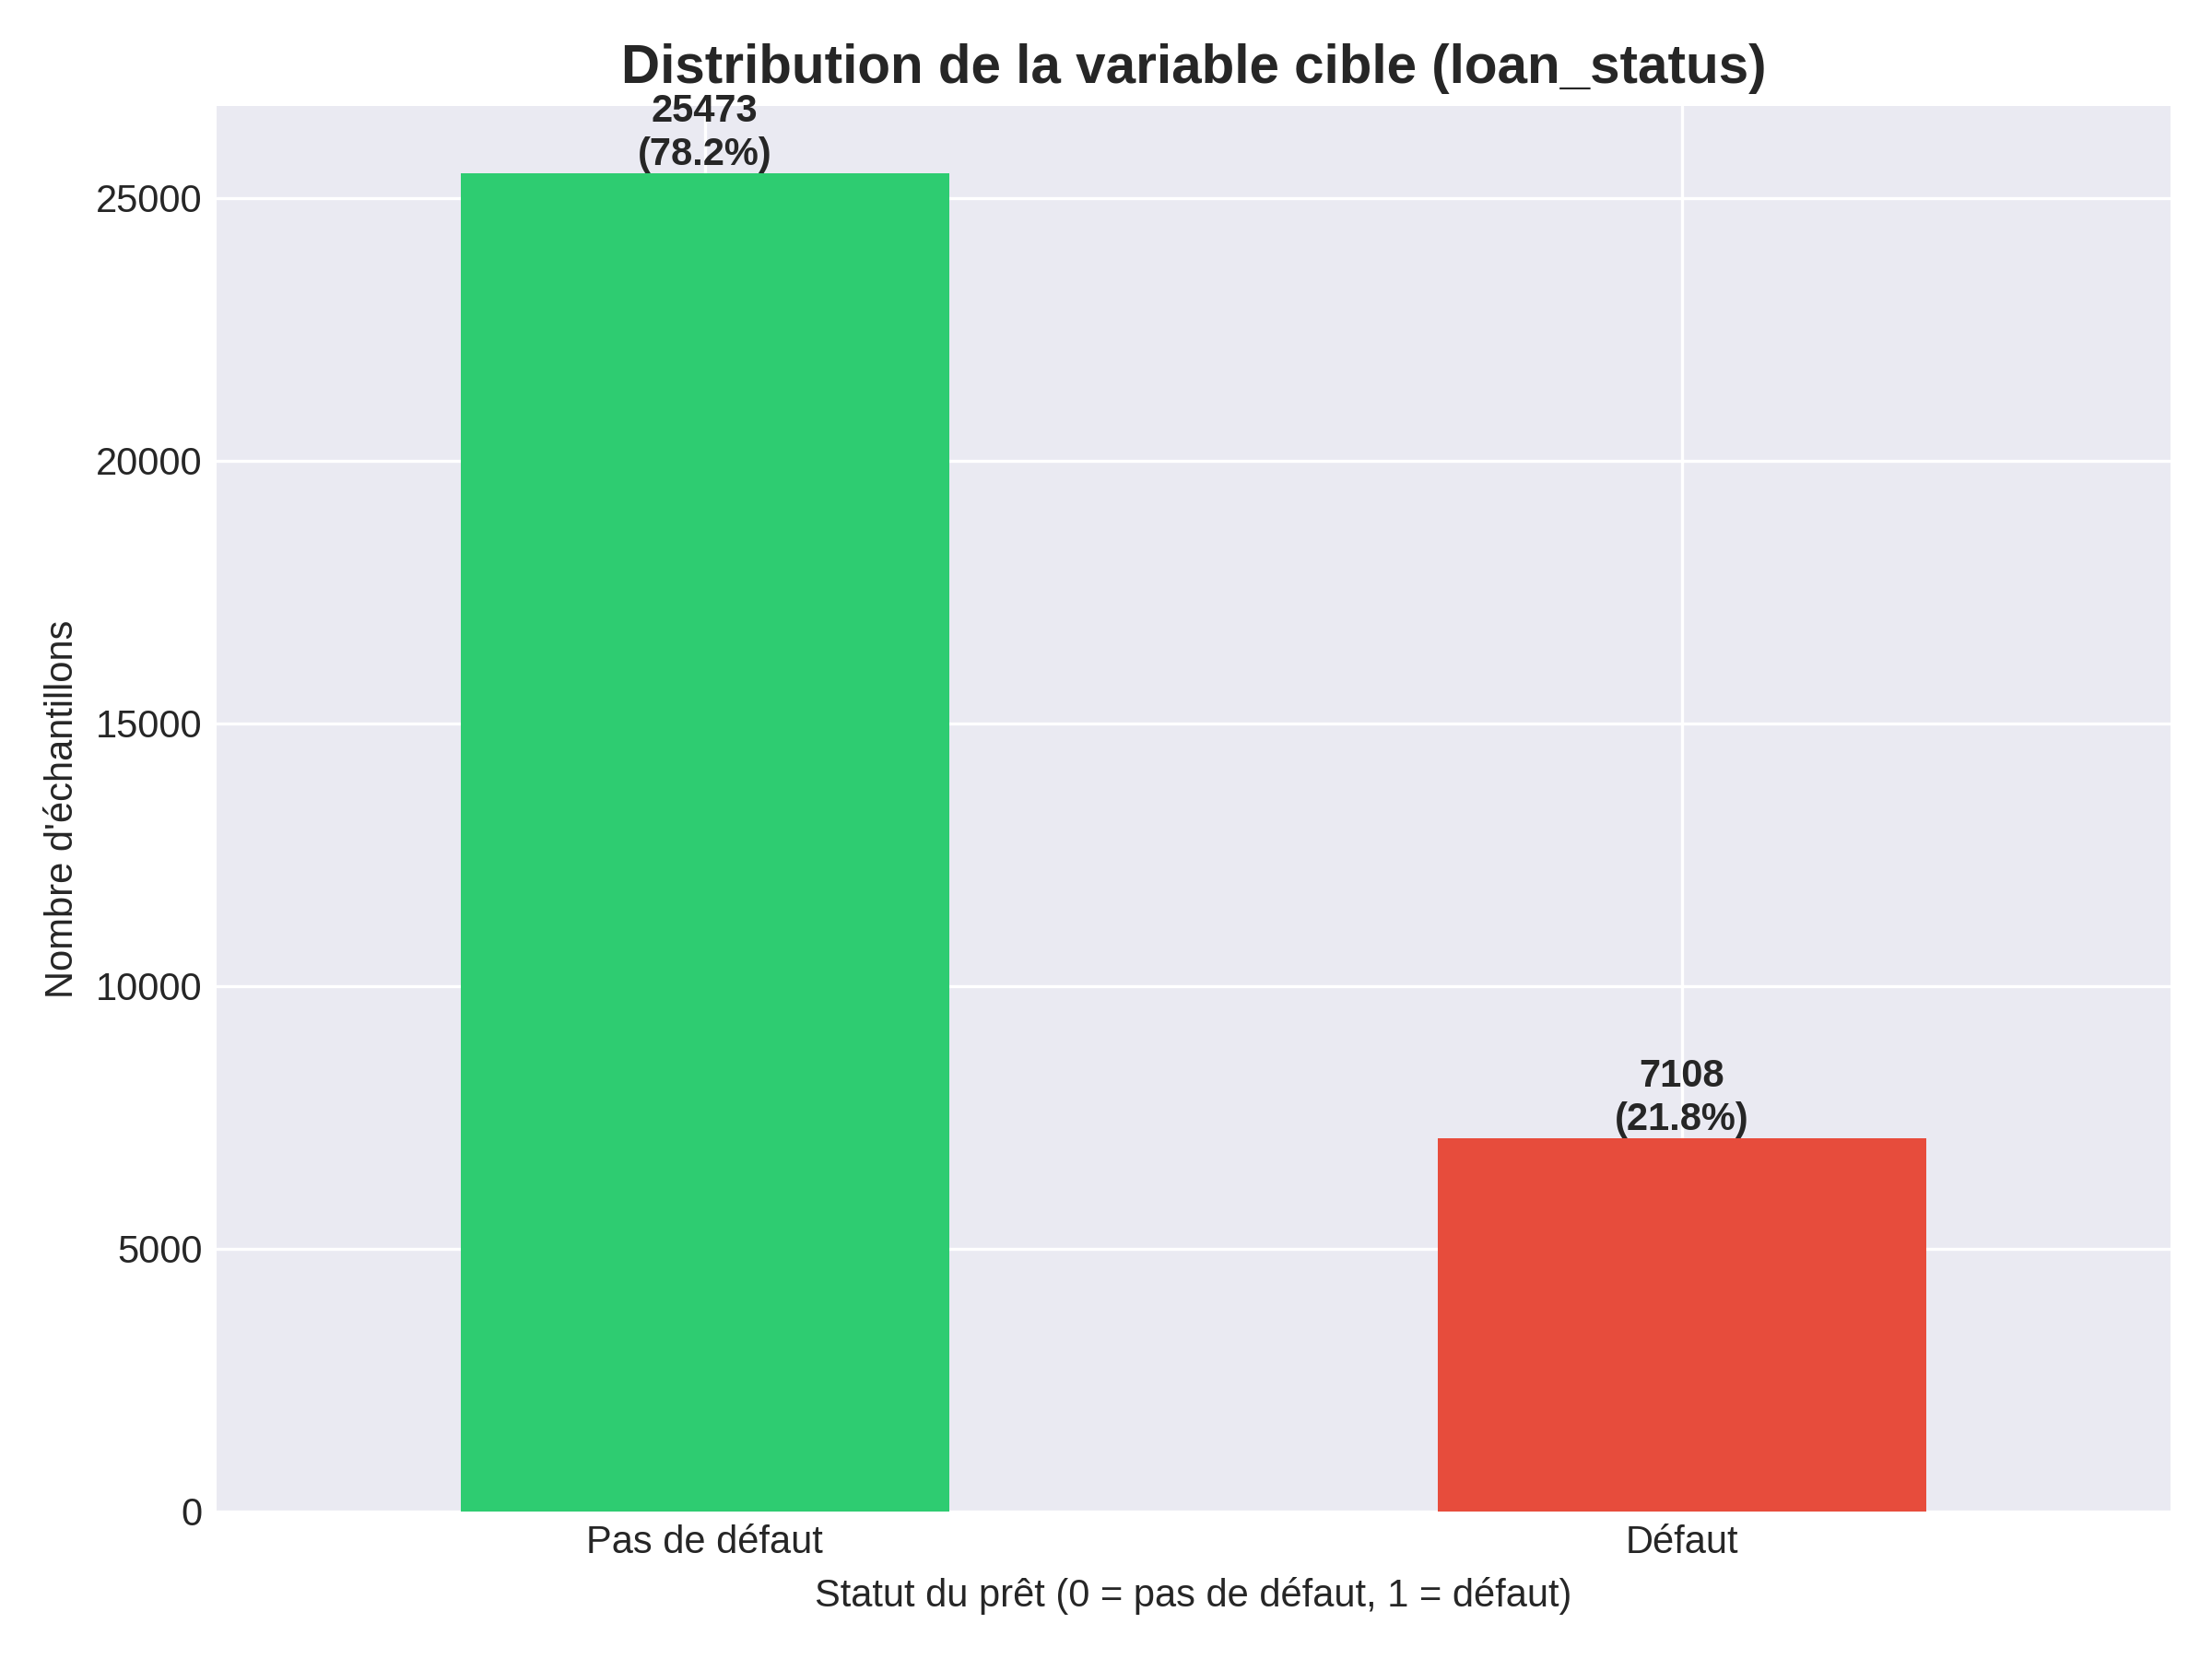
\includegraphics[width=0.72\textwidth]{target_distribution.png}
  \caption{Distribution de la variable cible \texttt{loan\_status} :
    le jeu de données est déséquilibré ($21{,}8\,\%$ de défauts).}
  \label{fig:target-distribution}
\end{figure}

\subsection{Problèmes identifiés lors de l'exploration}

L'analyse exploratoire (figures et statistiques disponibles dans
\texttt{data/stats/}) a mis en évidence trois problèmes à traiter avant
l'apprentissage :

\begin{itemize}
  \item \textbf{valeurs manquantes} : deux variables en contiennent,
    \texttt{loan\_int\_rate} ($9{,}6\,\%$ des lignes) et
    \texttt{person\_emp\_length} ($2{,}75\,\%$) ;
  \item \textbf{valeurs aberrantes} : quelques lignes contiennent des valeurs
    physiquement impossibles, comme des âges supérieurs à 120 ans ou une
    ancienneté d'emploi de 123 ans, manifestement des erreurs de saisie ;
  \item \textbf{déséquilibre des classes} : $78/22$, discuté ci-dessus.
\end{itemize}

L'exploration montre par ailleurs des corrélations attendues : le taux de
défaut croît fortement avec le grade du prêt (de A vers G) et avec la part du
revenu consacrée au remboursement (\texttt{loan\_percent\_income}), deux
variables dont on peut anticiper qu'elles joueront un rôle important dans les
modèles. Aucune colonne n'a été jugée inutile : les 11 variables explicatives
sont conservées.

% ======================================================================================
% Nom     : reports/latex/sections/04_pretraitement.tex
% Rôle    : Section décrivant le prétraitement des données.
% Auteur  : Maxime BRONNY
% Version : V1
% Cadre   : Réalisé dans le cadre du cours Techniques d'apprentissage artificiel
%           Master 1 Informatique Big Data
% Usage   : Fichier inclus dans main.tex lors de la compilation du rapport.
% ======================================================================================

\section{Prétraitement des données}
\label{sec:pretraitement}

Le prétraitement, qui s'appuie sur la bibliothèque pandas~\cite{mckinney2010pandas}
pour le chargement et la manipulation des données, est implémenté dans
\texttt{src/preprocessing.py} et \texttt{src/split\_data.py}. Un principe
structure l'ensemble :
\textbf{éviter toute fuite de données} (\emph{data leakage}). Tout paramètre
appris des données (médianes d'imputation, moyennes et écarts-types de
normalisation) est calculé \emph{uniquement} sur l'ensemble d'entraînement,
puis appliqué tel quel aux ensembles de validation et de test, qui jouent ainsi
pleinement leur rôle de données « jamais vues ».

\subsection{Nettoyage des valeurs aberrantes}

Les lignes physiquement impossibles identifiées lors de l'exploration sont
retirées : âge supérieur à 100 ans ou ancienneté d'emploi supérieure à 60 ans.
Seules \textbf{7 lignes sur 32\,581} sont concernées ($32\,574$ lignes
conservées). Nous ne touchons volontairement pas aux valeurs extrêmes mais
plausibles (revenus très élevés par exemple) : elles font partie de la vraie
distribution des données que les modèles doivent apprendre à gérer.

\subsection{Encodage des variables catégorielles}

Les quatre variables catégorielles sont converties en entiers par un
\emph{label encoding} à correspondance fixe, définie dans le code et non
apprise des données (tableau~\ref{tab:encodage}) ; l'encodage est donc
identique quel que soit le découpage.

\begin{table}[H]
  \centering
  \caption{Encodage des variables catégorielles.}
  \label{tab:encodage}
  \small
  \begin{tabular}{lp{8.5cm}}
    \toprule
    \textbf{Variable} & \textbf{Correspondance} \\
    \midrule
    \texttt{loan\_grade} & A$\to$0, B$\to$1, \ldots, G$\to$6 \\
    \texttt{cb\_person\_default\_on\_file} & N$\to$0, Y$\to$1 \\
    \texttt{person\_home\_ownership} & RENT$\to$0, OWN$\to$1, MORTGAGE$\to$2, OTHER$\to$3 \\
    \texttt{loan\_intent} & PERSONAL$\to$0, EDUCATION$\to$1, MEDICAL$\to$2,
      VENTURE$\to$3, HOMEIMPROVEMENT$\to$4, DEBTCONSOLIDATION$\to$5 \\
    \bottomrule
  \end{tabular}
\end{table}

Ce choix mérite justification. Pour \texttt{loan\_grade}, l'encodage entier est
naturel : la variable est \emph{ordinale} (A est un meilleur dossier que G) et
l'ordre numérique reflète un ordre réel. Pour
\texttt{cb\_person\_default\_on\_file}, binaire, l'encodage est sans ambiguïté.
Pour les deux variables \emph{nominales} (\texttt{person\_home\_ownership} et
\texttt{loan\_intent}), le label encoding introduit en revanche un ordre
artificiel entre modalités. Ce choix, hérité de la première version du projet
et conservé pour permettre la comparaison, reste acceptable pour l'arbre de
décision (qui peut isoler chaque modalité par divisions successives) et pour le
$k$-NN, mais constitue une limite pour la régression logistique ; nous y
revenons dans l'analyse critique (section~\ref{sec:analyse}).

\subsection{Découpage entraînement / validation / test}

Le jeu de données nettoyé est découpé en trois ensembles disjoints :
\textbf{70\,\% pour l'entraînement, 15\,\% pour la validation et 15\,\% pour le
test}, soit respectivement \textbf{22\,802, 4\,886 et 4\,886} observations.
Chaque ensemble a un rôle strictement distinct :

\begin{itemize}
  \item l'\textbf{entraînement} sert à apprendre les paramètres des modèles
    (poids de la régression, structure de l'arbre, instances mémorisées du
    $k$-NN) ;
  \item la \textbf{validation} sert \emph{uniquement} à choisir les
    hyperparamètres (seuil de décision, profondeur de l'arbre, nombre de
    voisins $k$) ;
  \item le \textbf{test} n'est utilisé qu'\emph{une seule fois}, à la toute
    fin, pour mesurer la performance de généralisation.
\end{itemize}

Cette séparation en trois est essentielle : si les hyperparamètres étaient
choisis directement sur le test, celui-ci ne mesurerait plus une capacité de
généralisation mais un ajustement indirect aux données d'évaluation, et les
performances rapportées seraient optimistes. La répartition $70/15/15$ offre un
bon compromis pour un jeu de cette taille : assez d'exemples d'entraînement
pour des modèles stables, et près de 5\,000 exemples dans chacun des deux
ensembles d'évaluation, ce qui donne des estimations fiables.

Le découpage est \textbf{stratifié} : il est effectué classe par classe, de
sorte que le taux de défaut ($21{,}8\,\%$) soit identique dans les trois
ensembles, comme le confirme la figure~\ref{fig:class-distribution}. Sans
stratification, un tirage aléatoire pourrait produire un ensemble de test non
représentatif. Le mélange utilise une graine aléatoire fixe ($42$), garantissant
la reproductibilité de toute l'expérience.

\begin{figure}[H]
  \centering
  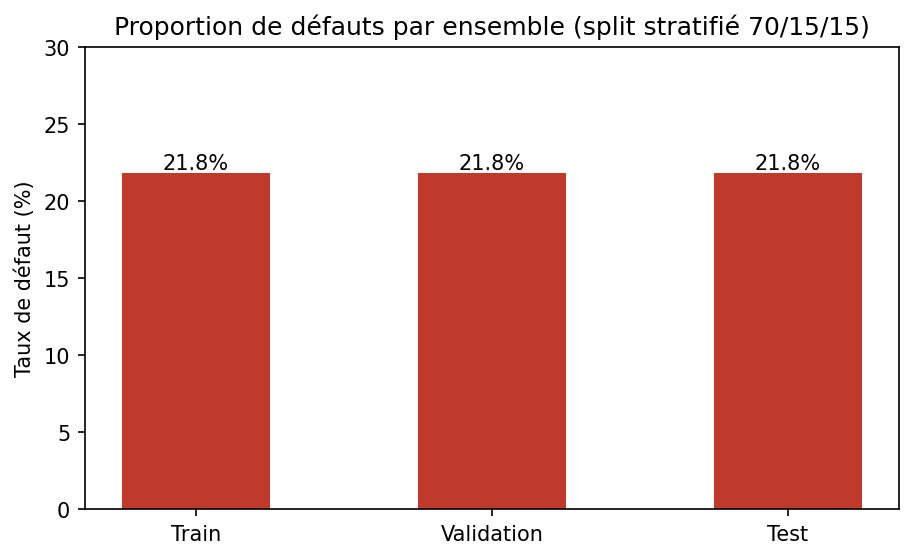
\includegraphics[width=0.7\textwidth]{class_distribution.png}
  \caption{Taux de défaut par ensemble après découpage stratifié $70/15/15$ :
    les trois ensembles conservent la même proportion de défauts
    ($21{,}8\,\%$).}
  \label{fig:class-distribution}
\end{figure}

\subsection{Imputation des valeurs manquantes}

Les valeurs manquantes des variables numériques sont remplacées par la
\textbf{médiane} de la variable, calculée sur le seul ensemble d'entraînement.
La médiane est préférée à la moyenne car elle est robuste aux valeurs extrêmes,
nombreuses dans les variables de revenu et de montant.

\subsection{Normalisation}

Les variables sont enfin standardisées (score $z$) :
\[
  x' = \frac{x - \mu_{\text{train}}}{\sigma_{\text{train}}},
\]
où $\mu_{\text{train}}$ et $\sigma_{\text{train}}$ sont la moyenne et
l'écart-type calculés sur l'entraînement. Cette normalisation est indispensable
pour deux des trois modèles : pour la régression logistique, elle conditionne
la vitesse et la stabilité de la descente de gradient ; pour le $k$-NN, elle
évite qu'une variable à grande échelle comme le revenu (de l'ordre de
$10^4$ à $10^5$) n'écrase toutes les autres dans le calcul des distances.
L'arbre de décision y est insensible (il ne compare que des seuils par
variable), mais reçoit les mêmes données afin de conserver un pipeline unique.

% ======================================================================================
% Nom     : reports/latex/sections/05_methodologie.tex
% Rôle    : Section décrivant la méthodologie et le protocole expérimental.
% Auteur  : Maxime BRONNY
% Version : V1
% Cadre   : Réalisé dans le cadre du cours Techniques d'apprentissage artificiel
%           Master 1 Informatique Big Data
% Usage   : Fichier inclus dans main.tex lors de la compilation du rapport.
% ======================================================================================

\section{Méthodologie}
\label{sec:methodologie}

\subsection{Choix des algorithmes}

Nous comparons trois méthodes de classification appartenant à trois familles
distinctes, ce qui donne à la comparaison un intérêt qui dépasse le simple
classement de performances :

\begin{itemize}
  \item la \textbf{régression logistique}, modèle \emph{linéaire}
    probabiliste : c'est la méthode de référence historique du credit scoring
    \cite{hosmer2000logistic}, interprétable (chaque variable reçoit un poids)
    et rapide ;
  \item l'\textbf{arbre de décision CART} \cite{breiman1984cart}, modèle
    \emph{non linéaire} à base de règles : il capture les interactions entre
    variables et produit des décisions lisibles (suites de tests
    « si\ldots{} alors ») ;
  \item les \textbf{$k$ plus proches voisins} \cite{cover1967knn}, méthode
    \emph{non paramétrique} à base d'instances : aucune phase d'apprentissage,
    la prédiction repose entièrement sur la similarité aux exemples connus.
\end{itemize}

Nous avons volontairement limité l'étude à trois méthodes maîtrisées de bout en
bout (toutes trois implémentées from scratch) plutôt que d'en survoler
davantage : l'objectif pédagogique est de comprendre finement chaque algorithme,
ses hyperparamètres et ses modes d'échec.

\subsection{Protocole expérimental}

Le protocole, entièrement automatisé par \texttt{main.py}, est identique pour
les trois modèles :

\begin{enumerate}
  \item \textbf{entraînement} sur les 22\,802 exemples du train ;
  \item \textbf{sélection des hyperparamètres sur la validation}
    (4\,886 exemples), avec le F1-score comme critère :
    \begin{itemize}
      \item seuil de décision (tous les modèles) : grille
        $\{0{,}3 ;\, 0{,}4 ;\, 0{,}5 ;\, 0{,}6\}$ ;
      \item profondeur maximale de l'arbre : grille $\{3, 5, 7, 9\}$ ;
      \item nombre de voisins du $k$-NN : grille $\{5, 11, 21, 31\}$ ;
    \end{itemize}
  \item \textbf{évaluation finale unique} sur les 4\,886 exemples du test ;
  \item \textbf{vérification} : chaque modèle est ré-entraîné avec son
    équivalent scikit-learn \cite{pedregosa2011sklearn} sur les mêmes données
    et avec des hyperparamètres équivalents, afin de valider la justesse de nos
    implémentations. Cette comparaison joue un rôle de contrôle qualité, pas de
    solution.
\end{enumerate}

Les grilles sont volontairement compactes : il s'agit de démontrer la démarche
de sélection sur validation, pas de mener une recherche exhaustive.
L'expérience complète est reproductible (graine fixe, une seule commande) et
s'exécute en une vingtaine de secondes.

\subsection{Métriques d'évaluation}

Toutes les métriques sont implémentées from scratch
(\texttt{src/metrics.py}). En notant TP, TN, FP, FN les vrais/faux
positifs/négatifs (la classe positive étant le défaut) :

\begin{align*}
  \text{accuracy} &= \frac{TP + TN}{TP + TN + FP + FN}
  & \text{précision} &= \frac{TP}{TP + FP} \\[4pt]
  \text{rappel} &= \frac{TP}{TP + FN}
  & F_1 &= \frac{2 \cdot \text{précision} \cdot \text{rappel}}
               {\text{précision} + \text{rappel}}
\end{align*}

Le choix de ces métriques découle directement du déséquilibre des classes :

\begin{itemize}
  \item l'\textbf{accuracy} donne une vue d'ensemble mais est insuffisante
    seule (prédire systématiquement la classe majoritaire donne déjà
    $78\,\%$) ;
  \item la \textbf{précision} mesure la fiabilité des alertes : parmi les
    défauts prédits, combien sont réels ;
  \item le \textbf{rappel} mesure la couverture : parmi les vrais défauts,
    combien sont détectés. C'est la métrique critique pour la banque,
    puisqu'un faux négatif correspond à un crédit accordé à un client qui ne
    remboursera pas ;
  \item le \textbf{F1-score}, moyenne harmonique des deux précédentes, sert de
    critère de sélection des hyperparamètres ;
  \item la \textbf{matrice de confusion} permet d'analyser la nature des
    erreurs ;
  \item la \textbf{courbe ROC} et l'\textbf{aire sous la courbe (AUC)}
    \cite{fawcett2006roc} comparent les modèles indépendamment du seuil de
    décision, à partir des probabilités prédites : l'AUC s'interprète comme la
    probabilité qu'un défaut tiré au hasard reçoive un score plus élevé qu'un
    non-défaut tiré au hasard.
\end{itemize}

Les métriques de régression (MAE, RMSE, $R^2$) et de partitionnement (inertie,
silhouette) ne sont pas pertinentes ici : le problème est une classification
supervisée, ni une régression ni un clustering.

% ======================================================================================
% Nom     : reports/latex/sections/06_algorithmes.tex
% Rôle    : Section présentant les algorithmes implémentés.
% Auteur  : Maxime BRONNY
% Version : V1
% Cadre   : Réalisé dans le cadre du cours Techniques d'apprentissage artificiel
%           Master 1 Informatique Big Data
% Usage   : Fichier inclus dans main.tex lors de la compilation du rapport.
% ======================================================================================

\section{Algorithmes implémentés}
\label{sec:algorithmes}

Les trois algorithmes sont implémentés from scratch en Python, avec NumPy pour
le calcul vectoriel, dans le module \texttt{src/models/}. Nous présentons pour
chacun le principe, les équations, les choix d'implémentation et les limites.

\subsection{Régression logistique}
\label{subsec:lr}

\paragraph{Principe.}
La régression logistique \cite{hosmer2000logistic} modélise directement la
probabilité de défaut comme une fonction du score linéaire
$z = \mathbf{w} \cdot \mathbf{x} + b$ passée dans la sigmoïde :
\[
  p(y = 1 \mid \mathbf{x}) = \sigma(z) = \frac{1}{1 + e^{-z}} .
\]
Les paramètres $\mathbf{w}$ et $b$ sont appris en minimisant l'entropie croisée
(\emph{log-loss}) sur l'ensemble d'entraînement :
\[
  J(\mathbf{w}, b) = -\frac{1}{n} \sum_{i=1}^{n}
    \left[ y_i \ln p_i + (1 - y_i) \ln (1 - p_i) \right],
\]
fonction convexe dont le minimum global est atteignable par descente de
gradient. Les gradients ont une forme remarquablement simple :
\[
  \frac{\partial J}{\partial \mathbf{w}} = \frac{1}{n} X^{\top}(\mathbf{p} - \mathbf{y}),
  \qquad
  \frac{\partial J}{\partial b} = \frac{1}{n} \sum_{i=1}^{n} (p_i - y_i).
\]

\paragraph{Implémentation.}
Notre implémentation (\texttt{src/models/logistic\_regression.py}) utilise une
descente de gradient \emph{full batch} : à chaque itération, le gradient est
calculé sur tout l'ensemble d'entraînement en une seule opération matricielle.
Deux détails numériques méritent mention : la sigmoïde est calculée par deux
formules équivalentes selon le signe de $z$ afin d'éviter tout dépassement de
capacité de l'exponentielle, et les probabilités sont bornées avant le
logarithme pour éviter $\ln 0$. Les hyperparamètres d'optimisation sont un taux
d'apprentissage de $0{,}1$ et $1\,000$ itérations, sur données normalisées. La
figure~\ref{fig:lr-cost} montre la décroissance régulière de la log-loss : la
descente de gradient converge sans oscillation, signe d'un taux d'apprentissage
bien dimensionné.

\begin{figure}[H]
  \centering
  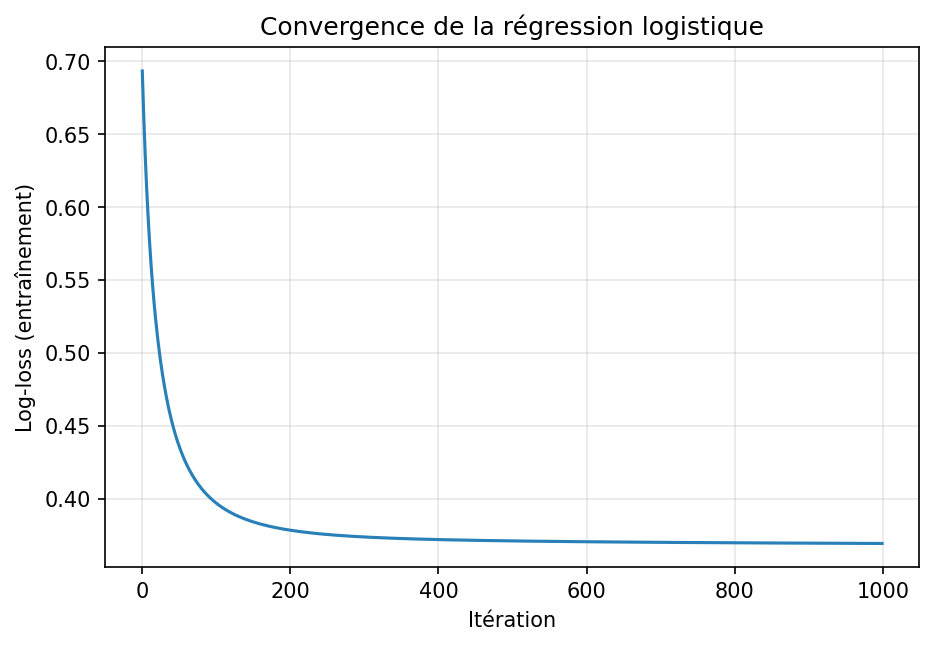
\includegraphics[width=0.68\textwidth]{lr_cost_curve.png}
  \caption{Convergence de la descente de gradient : décroissance de la
    log-loss sur l'ensemble d'entraînement ($1\,000$ itérations, taux
    d'apprentissage $0{,}1$).}
  \label{fig:lr-cost}
\end{figure}

Le seuil qui convertit la probabilité en classe est traité comme un
hyperparamètre choisi sur la validation ; la valeur retenue, $0{,}3$, est
inférieure au seuil naïf de $0{,}5$ : en présence de classes déséquilibrées,
abaisser le seuil augmente le rappel, ce qui est cohérent avec le coût élevé
des faux négatifs.

\paragraph{Limites.}
La frontière de décision reste un hyperplan : les interactions entre variables
(un même taux d'endettement n'a pas le même sens selon le grade du dossier) ne
sont pas modélisées. Le modèle est de plus pénalisé par l'encodage ordinal des
variables nominales, qui lui impose un ordre arbitraire.

\subsection{Arbre de décision CART}
\label{subsec:dt}

\paragraph{Principe.}
L'algorithme CART \cite{breiman1984cart} construit un arbre binaire par
partitionnement récursif. À chaque n\oe ud, il cherche le couple (variable,
seuil) qui sépare le mieux les exemples, au sens de l'impureté de Gini : pour
un groupe contenant une proportion $p$ de défauts, $G = 2p(1-p)$, nulle pour un
groupe pur et maximale pour un mélange $50/50$. Le couple retenu minimise la
moyenne pondérée des impuretés des deux groupes enfants. La construction
s'arrête quand le n\oe ud est pur, trop petit, ou que la profondeur maximale
est atteinte ; chaque feuille prédit alors la proportion de défauts des
exemples qu'elle contient, interprétable comme une probabilité.

\paragraph{Implémentation.}
La difficulté pratique est le coût de la recherche du meilleur seuil. Notre
implémentation (\texttt{src/models/decision\_tree.py}) la vectorise : pour
chaque variable, les valeurs sont triées et les sommes cumulées des étiquettes
donnent, pour \emph{toutes} les positions de coupure possibles à la fois, la
proportion de défauts de part et d'autre, et donc le Gini de tous les seuils
candidats en une seule passe NumPy, sans boucle Python sur les seuils. Cette
vectorisation rend l'entraînement quasi instantané sur 22\,802 exemples. Deux
garde-fous limitent le surapprentissage : un n\oe ud n'est divisé que s'il
contient au moins 20 exemples, et toute feuille doit en contenir au moins 5.
La profondeur maximale, hyperparamètre principal, est choisie sur la
validation ; l'arbre retenu a une profondeur de $7$ et compte $105$ n\oe uds.

\paragraph{Limites.}
Un arbre seul est un modèle instable : une perturbation des données
d'entraînement peut changer les premières divisions et, par effet de cascade,
toute la structure. Sans limite de profondeur, il mémoriserait le bruit du
train ; le contrôle par la validation est donc indispensable. Enfin, sa
frontière de décision « en escalier » approxime grossièrement les relations
continues douces.

\subsection{$k$ plus proches voisins ($k$-NN)}
\label{subsec:knn}

\paragraph{Principe.}
Le $k$-NN \cite{cover1967knn} ne construit aucun modèle : l'« apprentissage »
consiste à mémoriser l'ensemble d'entraînement. Pour classer un nouvel exemple,
on calcule sa distance euclidienne à tous les exemples mémorisés, on retient
les $k$ plus proches et l'on prédit la proportion de défauts parmi eux. Le
paramètre $k$ règle le compromis biais-variance : petit, la décision est locale
mais bruitée ; grand, elle est lissée mais peut noyer les structures locales.

\paragraph{Implémentation.}
La difficulté est ici la mémoire : la matrice complète des distances entre les
4\,886 exemples de test et les 22\,802 exemples d'entraînement occuperait de
l'ordre de 900~Mo. Notre implémentation (\texttt{src/models/knn.py}) procède
donc par paquets de quelques centaines d'exemples. Deux optimisations
classiques sont utilisées : le développement
$\lVert a - b \rVert^2 = \lVert a \rVert^2 + \lVert b \rVert^2 - 2\,a \cdot b$,
dont le terme $\lVert a \rVert^2$, constant pour un exemple donné, peut être
omis car il ne change pas l'ordre des voisins ; et la sélection des $k$ plus
petites distances par \texttt{np.argpartition}, en temps linéaire, au lieu d'un
tri complet. La valeur retenue sur la validation est $k = 31$.

\paragraph{Limites.}
Toute la charge de calcul est reportée à la prédiction, qui parcourt
l'ensemble d'entraînement complet pour chaque exemple, ce qui est rédhibitoire
pour un système temps réel à fort trafic sans structures d'index dédiées. La méthode
est par ailleurs très sensible à l'échelle des variables (d'où la
normalisation) et sa pertinence se dégrade en haute dimension.

% ======================================================================================
% Nom     : reports/latex/sections/07_resultats.tex
% Rôle    : Section présentant les résultats expérimentaux.
% Auteur  : Maxime BRONNY
% Version : V1
% Cadre   : Réalisé dans le cadre du cours Techniques d'apprentissage artificiel
%           Master 1 Informatique Big Data
% Usage   : Fichier inclus dans main.tex lors de la compilation du rapport.
% ======================================================================================

\section{Résultats}
\label{sec:resultats}

% Toutes les valeurs de cette section proviennent de l'exécution réelle du
% pipeline (python3 main.py, 12/06/2026, split 70/15/15 stratifié, seed 42).
% Source : results/metrics.json et results/sklearn_comparison.json.

\subsection{Sélection des hyperparamètres sur la validation}

Le tableau~\ref{tab:validation} retrace la sélection effectuée sur l'ensemble
de validation (critère : F1-score). Pour l'arbre, le F1 progresse nettement de
la profondeur 3 à la profondeur 7, puis recule légèrement à 9 : au-delà de 7,
la complexité supplémentaire n'apporte plus de pouvoir prédictif généralisable.
Pour le $k$-NN, le F1 est remarquablement stable sur la grille, signe que la
décision dépend peu du voisinage exact au-delà d'une dizaine de voisins.

\begin{table}[H]
  \centering
  \caption{Sélection des hyperparamètres sur l'ensemble de validation
    (F1-score ; en gras, la configuration retenue).}
  \label{tab:validation}
  \begin{tabular}{llcc}
    \toprule
    \textbf{Modèle} & \textbf{Configuration} & \textbf{Seuil optimal} & \textbf{F1 (validation)} \\
    \midrule
    Régression logistique & lr $=0{,}1$, $1\,000$ it. & \textbf{0,3} & \textbf{0,625} \\
    \midrule
    \multirow{4}{*}{Arbre de décision}
      & profondeur 3 & 0,3 & 0,728 \\
      & profondeur 5 & 0,3 & 0,776 \\
      & \textbf{profondeur 7} & \textbf{0,6} & \textbf{0,819} \\
      & profondeur 9 & 0,6 & 0,817 \\
    \midrule
    \multirow{4}{*}{$k$-NN}
      & $k = 5$  & 0,5 & 0,683 \\
      & $k = 11$ & 0,4 & 0,695 \\
      & $k = 21$ & 0,3 & 0,692 \\
      & $\boldsymbol{k = 31}$ & \textbf{0,3} & \textbf{0,695} \\
    \bottomrule
  \end{tabular}
\end{table}

\subsection{Performances sur l'ensemble de test}

Le tableau~\ref{tab:resultats-test} présente l'évaluation finale, réalisée une
seule fois sur l'ensemble de test.

\begin{table}[H]
  \centering
  \caption{Métriques des trois modèles sur l'ensemble de test
    (4\,886 exemples). Hyperparamètres choisis sur la validation.}
  \label{tab:resultats-test}
  \begin{tabular}{lccccc}
    \toprule
    \textbf{Modèle} & \textbf{Accuracy} & \textbf{Précision} & \textbf{Rappel}
      & \textbf{F1-score} & \textbf{AUC-ROC} \\
    \midrule
    Régression logistique (seuil 0,3)        & 0,820 & 0,573 & 0,690 & 0,626 & 0,848 \\
    Arbre de décision (prof.\ 7, seuil 0,6)  & \textbf{0,931} & \textbf{0,977}
      & \textbf{0,703} & \textbf{0,817} & \textbf{0,909} \\
    $k$-NN ($k=31$, seuil 0,3)               & 0,862 & 0,683 & 0,684 & 0,683 & 0,877 \\
    \bottomrule
  \end{tabular}
\end{table}

La hiérarchie est nette et cohérente sur toutes les métriques : \textbf{l'arbre
de décision domine}, suivi du $k$-NN, puis de la régression logistique. L'arbre
atteint un F1 de $0{,}817$ et une AUC de $0{,}909$ ; son avance la plus
spectaculaire concerne la précision ($0{,}977$) : lorsqu'il prédit un défaut,
il se trompe très rarement. Les trois modèles plafonnent en revanche à un
rappel compris entre $0{,}69$ et $0{,}70$ : quel que soit le modèle, environ
$30\,\%$ des défauts échappent à la détection. Nous y revenons dans l'analyse
critique.

\subsection{Matrices de confusion}

\begin{figure}[H]
  \centering
  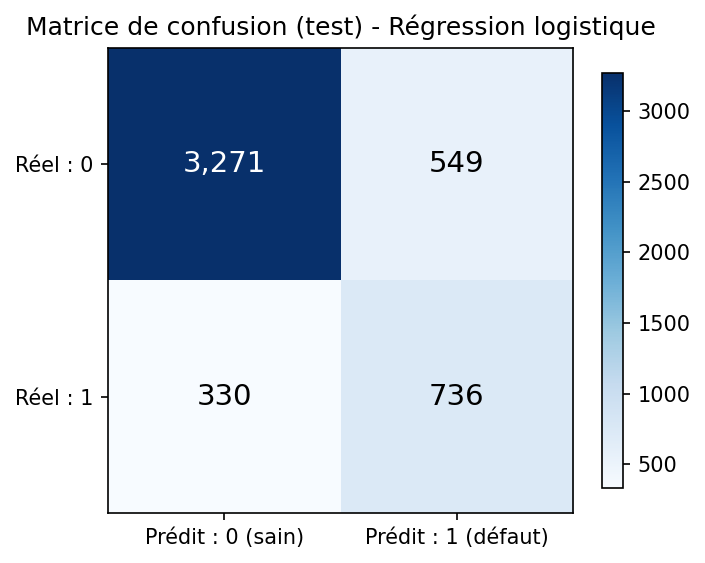
\includegraphics[width=0.32\textwidth]{lr_confusion_matrix.png}\hfill
  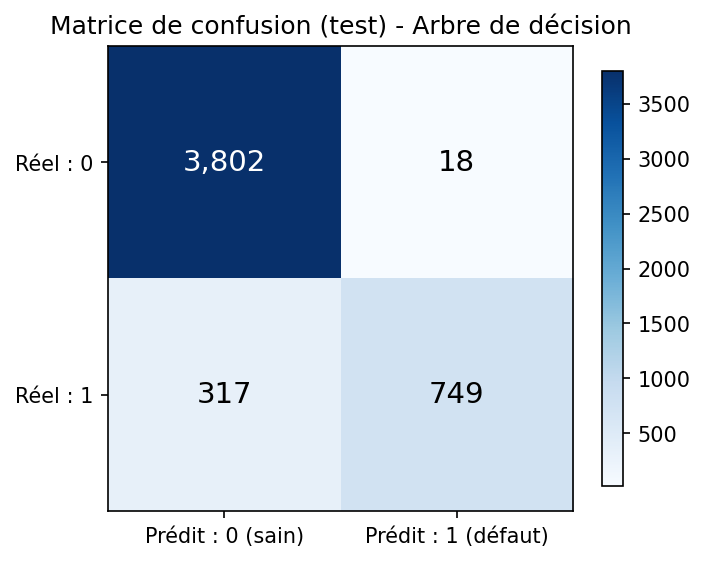
\includegraphics[width=0.32\textwidth]{dt_confusion_matrix.png}\hfill
  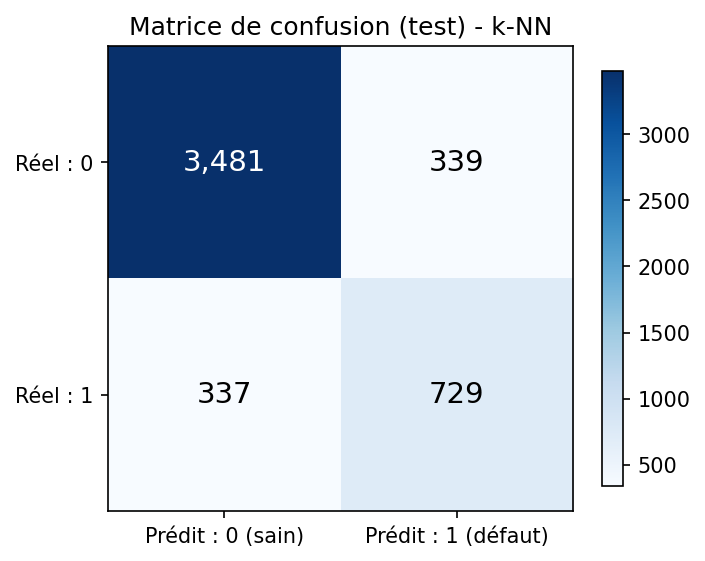
\includegraphics[width=0.32\textwidth]{knn_confusion_matrix.png}
  \caption{Matrices de confusion sur l'ensemble de test : régression
    logistique (gauche), arbre de décision (centre), $k$-NN (droite).}
  \label{fig:confusion-matrices}
\end{figure}

La lecture détaillée des matrices (figure~\ref{fig:confusion-matrices})
éclaire les différences de comportement. Sur les 4\,886 dossiers de test
(dont 1\,066 défauts) :

\begin{itemize}
  \item l'\textbf{arbre} ne commet que \textbf{18 faux positifs} (bons clients
    refusés) pour 749 défauts détectés, soit un profil très « prudent dans
    l'alerte » ; ses erreurs sont presque exclusivement des faux négatifs
    (317) ;
  \item la \textbf{régression logistique}, avec son seuil abaissé à $0{,}3$,
    détecte un nombre comparable de défauts (736) mais au prix de 549 faux
    positifs, soit trente fois plus que l'arbre ;
  \item le \textbf{$k$-NN} occupe une position intermédiaire (729 défauts
    détectés, 339 faux positifs).
\end{itemize}

Autrement dit, à rappel quasi égal, les trois modèles se distinguent presque
uniquement par leur taux de fausses alertes. C'est ce qui explique l'écart
de précision et donc de F1.

\subsection{Courbes ROC et comparaison globale}

\begin{figure}[H]
  \centering
  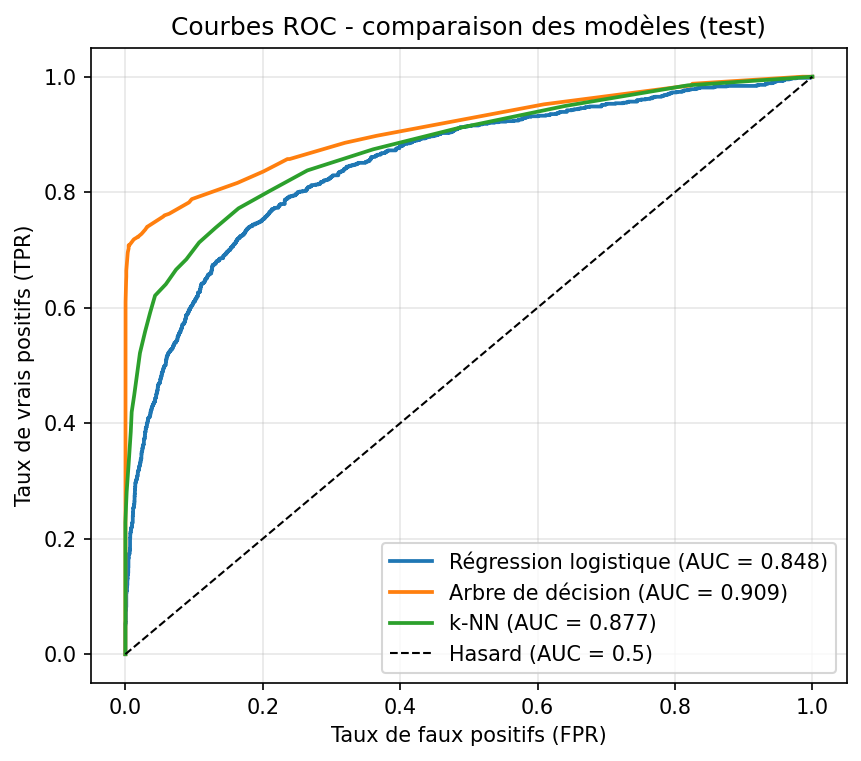
\includegraphics[width=0.75\textwidth]{roc_curves_comparison.png}
  \caption{Courbes ROC des trois modèles sur l'ensemble de test.
    AUC : arbre de décision $0{,}909$ ; $k$-NN $0{,}877$ ;
    régression logistique $0{,}848$.}
  \label{fig:roc}
\end{figure}

Les courbes ROC (figure~\ref{fig:roc}) confirment la hiérarchie
indépendamment du seuil de décision : la courbe de l'arbre domine celle du
$k$-NN, qui domine celle de la régression logistique, sur la quasi-totalité de
la plage de fonctionnement. Les trois modèles sont très au-dessus de la
diagonale du hasard (AUC $0{,}5$). La figure~\ref{fig:models-comparison}
récapitule les cinq métriques. L'ensemble des figures de ce rapport est produit
avec Matplotlib~\cite{hunter2007matplotlib}.

\begin{figure}[H]
  \centering
  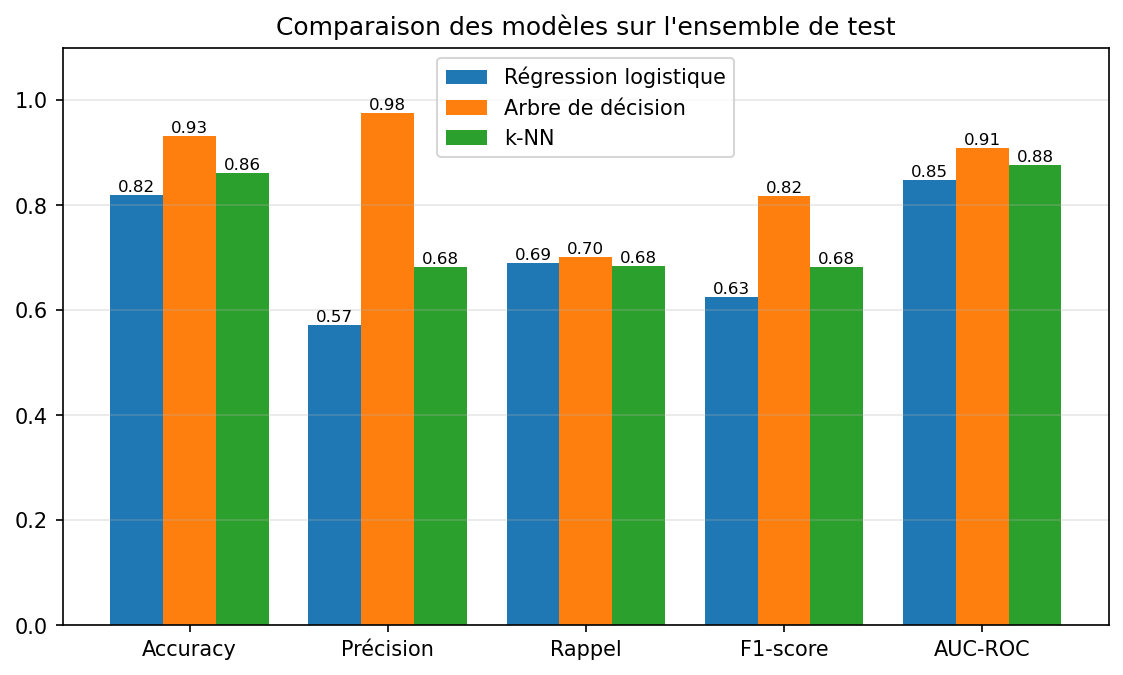
\includegraphics[width=0.92\textwidth]{models_comparison.png}
  \caption{Comparaison des cinq métriques sur l'ensemble de test.}
  \label{fig:models-comparison}
\end{figure}

\subsection{Validation des implémentations avec scikit-learn}

Pour vérifier la justesse de nos implémentations, chaque modèle a été
ré-entraîné avec son équivalent scikit-learn sur exactement les mêmes ensembles
et avec des hyperparamètres équivalents (tableau~\ref{tab:sklearn}).

\begin{table}[H]
  \centering
  \caption{Vérification des implémentations from scratch : AUC sur l'ensemble
    de test, comparée à scikit-learn.}
  \label{tab:sklearn}
  \begin{tabular}{lccc}
    \toprule
    \textbf{Modèle} & \textbf{AUC from scratch} & \textbf{AUC scikit-learn}
      & \textbf{Écart} \\
    \midrule
    Régression logistique & 0,8479 & 0,8483 & $-0{,}0005$ \\
    Arbre de décision     & 0,9086 & 0,9086 & $0{,}0000$ \\
    $k$-NN                & 0,8772 & 0,8772 & $0{,}0000$ \\
    \bottomrule
  \end{tabular}
\end{table}

L'arbre et le $k$-NN obtiennent une AUC \emph{identique} à celle de
scikit-learn, et l'écart de la régression logistique ($5 \times 10^{-4}$)
s'explique par les différences d'optimiseur (notre descente de gradient pure
contre L-BFGS) et par la régularisation L2 activée par défaut dans
scikit-learn. Ces écarts négligeables valident nos trois implémentations.
L'ensemble du pipeline, comprenant le prétraitement, l'entraînement des trois
modèles, la sélection sur validation, l'évaluation et la génération des figures,
s'exécute en une vingtaine de secondes.

% ======================================================================================
% Nom     : reports/latex/sections/08_analyse_critique.tex
% Rôle    : Section d'analyse critique des résultats.
% Auteur  : Maxime BRONNY
% Version : V1
% Cadre   : Réalisé dans le cadre du cours Techniques d'apprentissage artificiel
%           Master 1 Informatique Big Data
% Usage   : Fichier inclus dans main.tex lors de la compilation du rapport.
% ======================================================================================

\section{Analyse critique}
\label{sec:analyse}

\subsection{Pourquoi l'arbre de décision domine-t-il ?}

La supériorité de l'arbre s'explique par la nature du problème. Le risque de
crédit repose sur des \emph{interactions} entre variables : un taux
d'endettement de $30\,\%$ n'a pas la même signification pour un dossier de
grade A que pour un grade F, et un antécédent de défaut ne pèse pas pareil
selon le revenu. La régression logistique, qui additionne des contributions
indépendantes des variables, ne peut pas représenter ces effets croisés ; sa
frontière de décision reste un hyperplan, et son AUC plafonne à $0{,}848$.
L'arbre, en enchaînant des tests conditionnels (d'abord le grade, puis le taux
d'endettement \emph{dans} chaque branche, etc.), modélise naturellement ces
interactions, d'où son AUC de $0{,}909$ et surtout sa précision de
$0{,}977$. Le $k$-NN, qui capte la structure locale des données sans la
modéliser explicitement, se place logiquement entre les deux.

\subsection{L'apport mesurable de l'ensemble de validation}

Le réglage du seuil de décision sur la validation illustre concrètement
l'intérêt du découpage en trois ensembles. Pour la régression logistique, le
seuil retenu ($0{,}3$) relève le rappel à $0{,}69$ là où le seuil naïf de
$0{,}5$ (celui de la première version du projet) donnait un F1 d'environ
$0{,}50$ ; le F1 atteint désormais $0{,}626$, soit un gain d'environ douze
points obtenu \emph{sans toucher au modèle}, simplement par un protocole
expérimental plus rigoureux. À l'inverse, l'arbre préfère un seuil élevé
($0{,}6$) qui filtre les feuilles incertaines et lui donne sa précision
remarquable. Le seuil optimal est donc bien une propriété propre à chaque
modèle, qu'il serait incorrect de fixer uniformément à $0{,}5$.

\subsection{Surapprentissage : un risque contrôlé}

La comparaison des métriques d'entraînement et de test
(\texttt{results/metrics.json}) montre des écarts très faibles : F1 de
$0{,}623$ (train) contre $0{,}626$ (test) pour la régression logistique,
$0{,}814$ contre $0{,}817$ pour l'arbre. Deux mécanismes y contribuent : les
garde-fous de l'arbre (taille minimale des n\oe uds et des feuilles) et surtout
la sélection de la profondeur sur la validation, qui a écarté la profondeur 9
(F1 de validation $0{,}817$ contre $0{,}819$ pour la profondeur 7) ; le début
de surapprentissage a donc été détecté et évité par le protocole lui-même. Le
$k$-NN présente l'écart le plus visible (AUC $0{,}907$ en train contre
$0{,}877$ en test), comportement attendu d'une méthode à base d'instances
évaluée sur ses propres exemples mémorisés ; l'écart reste modéré grâce au
lissage d'un $k$ élevé ($31$).

\subsection{Le rappel, limite commune aux trois modèles}

Le résultat le plus instructif n'est pas la hiérarchie des modèles mais leur
plafond commun : environ $30\,\%$ des défauts ne sont détectés par aucun
modèle, alors même que leurs familles algorithmiques sont très différentes.
Cela suggère que la limite ne vient pas des algorithmes mais de
l'\emph{information disponible} : une partie des défauts n'est simplement pas
prévisible à partir des onze variables du dossier de crédit (accidents de la
vie, perte d'emploi postérieure à l'octroi, etc.). Pour une banque, ce constat
est important : améliorer encore le modèle rapporterait moins que collecter des
variables plus informatives.

\subsection{Points forts et réserves sur la qualité des données}

Au crédit du travail : un protocole sans fuite de données (paramètres de
prétraitement appris sur le seul entraînement), une évaluation finale unique,
des implémentations validées par une référence externe (écart d'AUC
$\leq 5 \times 10^{-4}$), une expérience entièrement reproductible (graine
fixe) et couverte par onze tests automatisés.

Côté réserves : l'imputation par la médiane de \texttt{loan\_int\_rate}
(près de $10\,\%$ de valeurs manquantes) lisse l'information d'une variable
probablement liée au risque ; le label encoding impose un ordre artificiel aux
deux variables nominales, ce qui pénalise principalement la régression
logistique, et une partie de son retard pourrait venir de là plutôt que de sa
linéarité seule ; enfin, le déséquilibre des classes n'est traité que par le
réglage du seuil, sans ré-échantillonnage ni pondération.

% ======================================================================================
% Nom     : reports/latex/sections/09_limites_ameliorations.tex
% Rôle    : Section présentant les limites et les améliorations possibles.
% Auteur  : Maxime BRONNY
% Version : V1
% Cadre   : Réalisé dans le cadre du cours Techniques d'apprentissage artificiel
%           Master 1 Informatique Big Data
% Usage   : Fichier inclus dans main.tex lors de la compilation du rapport.
% ======================================================================================

\section{Limites et améliorations possibles}
\label{sec:limites}

Les limites identifiées dans l'analyse critique dessinent directement les
améliorations envisageables, classées ici de la plus simple à la plus
structurante.

\paragraph{Encodage one-hot des variables nominales.}
Remplacer le label encoding de \texttt{loan\_intent} et
\texttt{person\_home\_ownership} par un encodage one-hot (une colonne binaire
par modalité) supprimerait l'ordre artificiel entre modalités. Le bénéfice
attendu concerne d'abord la régression logistique, qui pourrait attribuer un
poids propre à chaque modalité ; le coût est minime (quelques colonnes
supplémentaires).

\paragraph{Régularisation L2.}
Notre régression logistique ne comporte aucune pénalité sur les poids, là où
scikit-learn en applique une par défaut. C'est l'une des sources du petit
écart observé. Ajouter un terme $\lambda \lVert \mathbf{w} \rVert^2$ au coût
(et $2\lambda\mathbf{w}$ au gradient) est immédiat et stabiliserait le modèle,
notamment après un passage au one-hot qui augmente le nombre de colonnes.

\paragraph{Validation croisée $k$-fold.}
Le découpage unique $70/15/15$, même stratifié et à graine fixe, fournit une
estimation ponctuelle des performances. Une validation croisée à $k$ blocs
donnerait une moyenne et un écart-type pour chaque métrique, permettant de dire
si l'écart entre deux modèles est significatif. Le coût, à savoir $k$
entraînements au lieu d'un, resterait négligeable ici (le pipeline complet dure
une vingtaine de secondes).

\paragraph{Recherche d'hyperparamètres élargie.}
Les grilles utilisées sont volontairement compactes (quatre valeurs par
hyperparamètre). Une grille plus fine (profondeurs intermédiaires,
\texttt{min\_samples\_leaf} variable, $k$ pairs/impairs, seuils au pas de
$0{,}05$) pourrait apporter quelques points supplémentaires, au prix d'un
temps de calcul encore raisonnable.

\paragraph{Forêt aléatoire.}
L'extension la plus naturelle du travail : entraîner plusieurs arbres CART sur
des échantillons bootstrap avec sous-échantillonnage des variables, et moyenner
leurs prédictions. Notre implémentation de CART constitue déjà la brique de
base ; la forêt réduirait l'instabilité de l'arbre seul, sa principale
faiblesse structurelle.

\paragraph{Traitement explicite du déséquilibre.}
Compléter le réglage du seuil par une pondération des classes dans la fonction
de coût, ou par un ré-échantillonnage de l'entraînement (sur-échantillonnage
des défauts ou sous-échantillonnage des remboursements), pourrait relever le
rappel (la métrique critique) au prix d'un arbitrage à documenter sur la
précision.

\paragraph{Choix du seuil par coûts métier.}
Le F1-score accorde le même poids à la précision et au rappel. Une banque
préférerait minimiser un coût total explicite, de la forme
$C = c_{FN} \cdot FN + c_{FP} \cdot FP$ avec $c_{FN} \gg c_{FP}$ : le seuil
optimal s'en déduirait directement, et la comparaison des modèles se ferait en
euros plutôt qu'en points de F1.

\paragraph{Visualisations complémentaires.}
Deux figures enrichiraient l'analyse : la courbe précision-rappel, plus
informative que la ROC en présence de déséquilibre, et l'importance des
variables de l'arbre (réduction totale de Gini par variable), qui relierait
les performances aux intuitions métier de la section~\ref{sec:donnees}.

% ======================================================================================
% Nom     : reports/latex/sections/10_conclusion.tex
% Rôle    : Section de conclusion du rapport.
% Auteur  : Maxime BRONNY
% Version : V1
% Cadre   : Réalisé dans le cadre du cours Techniques d'apprentissage artificiel
%           Master 1 Informatique Big Data
% Usage   : Fichier inclus dans main.tex lors de la compilation du rapport.
% ======================================================================================

\section{Conclusion}
\label{sec:conclusion}

\subsection{Bilan du travail réalisé}

Ce projet a permis de construire un pipeline d'apprentissage automatique
complet et reproductible pour la prédiction du risque de crédit bancaire :
chargement et nettoyage de 32\,581 dossiers, encodage des variables
catégorielles, découpage stratifié en trois ensembles ($70/15/15$), imputation
et normalisation sans fuite de données, entraînement de trois modèles de
familles différentes implémentés from scratch en Python, sélection des
hyperparamètres sur l'ensemble de validation, évaluation finale unique sur
l'ensemble de test, et génération automatique des métriques
(\texttt{results/metrics.json}) et des figures. L'ensemble s'exécute en une
seule commande et une vingtaine de secondes, et la justesse des trois
implémentations a été validée par comparaison avec scikit-learn (écarts d'AUC
inférieurs ou égaux à $5 \times 10^{-4}$).

\subsection{Réponse à la problématique}

Oui, le risque de défaut est prédictible avec une fiabilité utile à partir des
seules caractéristiques du dossier, et la comparaison désigne clairement
\textbf{l'arbre de décision} comme le meilleur compromis : F1 de $0{,}817$,
AUC de $0{,}909$ et une précision de $0{,}977$ qui rend ses alertes presque
toujours fondées, devant le $k$-NN (F1 $0{,}683$) et la régression logistique
(F1 $0{,}626$). La réponse doit cependant être nuancée par le plafond commun
des trois modèles : environ $30\,\%$ des défauts restent indétectés, limite qui
semble tenir à l'information disponible dans les données plus qu'aux
algorithmes eux-mêmes. Un déploiement réel exigerait donc soit des variables
supplémentaires, soit l'acceptation explicite de ce risque résiduel.

\subsection{Intérêt de la migration vers Python}

La réécriture du projet, initialement développé en C, s'est révélée bien plus
qu'une traduction. Le passage à Python et NumPy a divisé la taille du code par
plusieurs fois et l'a rendu directement confrontable à une référence
(scikit-learn), ce que la version C ne permettait qu'imparfaitement. Surtout,
l'effort économisé sur la gestion de la mémoire a pu être réinvesti dans le
protocole expérimental : ajout d'un ensemble de validation dédié (dont
l'apport est mesurable : environ douze points de F1 gagnés sur la régression
logistique par le seul réglage du seuil), ajout d'une troisième méthode, et
couverture par des tests automatisés. La compréhension fine des algorithmes
n'a rien perdu au change, puisque chaque méthode reste implémentée from
scratch, équations à l'appui.

\subsection{Bilan personnel d'apprentissage}

% Bilan rédigé à la première personne - à ajuster avec tes propres mots si tu
% le souhaites.
Ce projet m'a d'abord appris ce que « implémenter from scratch » exige
réellement : écrire une sigmoïde, c'est facile ; écrire une sigmoïde qui ne
déborde pas numériquement, une recherche de seuil de Gini qui tient en quelques
opérations vectorisées, ou un $k$-NN qui ne sature pas la mémoire, c'est là que
se loge la vraie compréhension des algorithmes. J'ai ensuite mesuré à quel
point le protocole expérimental compte autant que les modèles : la distinction
validation/test, que je percevais comme une convention, a produit sous mes yeux
un gain de douze points de F1 et détecté un début de surapprentissage. Enfin,
travailler sur des classes déséquilibrées m'a définitivement guéri de lire une
accuracy au premier degré : c'est la matrice de confusion, lue avec les coûts
métier en tête, qui dit ce qu'un classifieur vaut vraiment.


% ============================================================================
% Bibliographie
% ============================================================================
% Bibliographie intégrée (thebibliography, sans BibTeX) : garantit des tirets
% simples dans les plages de pages et un contrôle direct de la présentation.
% Chaque référence a été vérifiée (auteurs, année, revue, pages, DOI/URL).
\clearpage
\phantomsection
\addcontentsline{toc}{section}{Bibliographie}
\begin{thebibliography}{10}

\bibitem{breiman1984cart}
Leo Breiman, Jerome Friedman, Richard Olshen et Charles Stone.
\newblock {\em Classification and Regression Trees}.
\newblock Wadsworth \& Brooks/Cole, 1984.
\newblock Ouvrage fondateur de l'arbre de décision CART implémenté dans le projet.

\bibitem{cover1967knn}
Thomas M. Cover et Peter E. Hart.
\newblock Nearest neighbor pattern classification.
\newblock {\em IEEE Transactions on Information Theory}, 13(1):21-27, 1967.
\newblock DOI~: \href{https://doi.org/10.1109/TIT.1967.1053964}{10.1109/TIT.1967.1053964}.
  Article fondateur de la méthode des $k$ plus proches voisins.

\bibitem{fawcett2006roc}
Tom Fawcett.
\newblock An introduction to {ROC} analysis.
\newblock {\em Pattern Recognition Letters}, 27(8):861-874, 2006.
\newblock DOI~: \href{https://doi.org/10.1016/j.patrec.2005.10.010}{10.1016/j.patrec.2005.10.010}.
  Référence sur la courbe ROC et l'AUC employées pour comparer les modèles.

\bibitem{harris2020numpy}
Charles R. Harris, K. Jarrod Millman, Stéfan J. van der Walt et al.
\newblock Array programming with {NumPy}.
\newblock {\em Nature}, 585(7825):357-362, 2020.
\newblock DOI~: \href{https://doi.org/10.1038/s41586-020-2649-2}{10.1038/s41586-020-2649-2}.
  Bibliothèque de calcul numérique, base de toutes les implémentations \emph{from scratch}.

\bibitem{hosmer2000logistic}
David W. Hosmer et Stanley Lemeshow.
\newblock {\em Applied Logistic Regression}.
\newblock John Wiley \& Sons, 2\textsuperscript{e} édition, 2000.
\newblock DOI~: \href{https://doi.org/10.1002/0471722146}{10.1002/0471722146}.
  Ouvrage de référence sur la régression logistique.

\bibitem{hunter2007matplotlib}
John D. Hunter.
\newblock Matplotlib: a 2{D} graphics environment.
\newblock {\em Computing in Science \& Engineering}, 9(3):90-95, 2007.
\newblock DOI~: \href{https://doi.org/10.1109/MCSE.2007.55}{10.1109/MCSE.2007.55}.
  Bibliothèque utilisée pour générer toutes les figures du rapport.

\bibitem{kaggle_credit_risk}
laotse.
\newblock Credit Risk Dataset - jeu de données de risque de crédit utilisé dans
  le projet (32\,581 dossiers, licence CC0).
\newblock Kaggle, 2020.
  \url{https://www.kaggle.com/datasets/laotse/credit-risk-dataset}.
  Consulté en juin 2026.

\bibitem{mckinney2010pandas}
Wes McKinney.
\newblock Data structures for statistical computing in {Python}.
\newblock {\em Proceedings of the 9th Python in Science Conference}, pages 56-61, 2010.
\newblock DOI~: \href{https://doi.org/10.25080/Majora-92bf1922-00a}{10.25080/Majora-92bf1922-00a}.
  Bibliothèque pandas, utilisée pour le chargement et la manipulation des données.

\bibitem{pedregosa2011sklearn}
Fabian Pedregosa, Gaël Varoquaux, Alexandre Gramfort et al.
\newblock Scikit-learn: machine learning in {Python}.
\newblock {\em Journal of Machine Learning Research}, 12:2825-2830, 2011.
\newblock \url{https://jmlr.org/papers/v12/pedregosa11a.html}.
  Bibliothèque utilisée uniquement pour vérifier les implémentations \emph{from scratch}.

\bibitem{python_psf}
Python Software Foundation.
\newblock Python - langage de programmation utilisé pour l'ensemble de
  l'implémentation du projet.
\newblock \url{https://www.python.org/}, 1991. Consulté en juin 2026.

\end{thebibliography}

\end{document}
